\documentclass{article}
\usepackage{amsmath}
\usepackage[margin=1.0 in]{geometry}

\usepackage{bbm}
\usepackage{booktabs}

\newcommand{\fabs}[1]{\mid {#1} \mid}

\newcommand{\bet}[1]{\llbracket {#1} \rrbracket^{\beta} }
\usepackage{stmaryrd}
\usepackage{graphicx}
\usepackage{tikz}
\usepackage{wrapfig}
\usepackage{makecell}

% \usepackage{mathabx}
\usepackage{amssymb,forest}

\usepackage{float}
\usepackage{MnSymbol}
\newlength\q
\newlength\smallCol
\newlength\argsLen
\setlength\q{\dimexpr .5\textwidth -2\tabcolsep}
\setlength\smallCol{\dimexpr .15\textwidth}
\setlength\argsLen{\dimexpr .2\textwidth}


\newcommand{\lto}{\mathbin{\to}}
\usepackage{booktabs}
\usepackage{enumitem} 
\usepackage{array}% for extended column definitions
\usepackage{graphicx}
\usepackage{verbatim}
\usepackage{tabto}
\newcommand{\ov}[2]{\ensuremath{\overset{\cdot {#2} \cdot}{#1}}}
\newcommand{\imp}{\rightarrow}

\usepackage{xstring}
\usepackage[german]{babel}
\usepackage[utf8]{inputenc}

\usepackage{lipsum}
\usepackage{listings}
\usepackage{color}

\definecolor{dkgreen}{rgb}{0,0.6,0}
\definecolor{gray}{rgb}{0.5,0.5,0.5}
\definecolor{mauve}{rgb}{0.58,0,0.82}

\lstset{frame=tb,
  language=Java,
  aboveskip=3mm,
  belowskip=3mm,
  showstringspaces=false,
  columns=flexible,
  basicstyle={\small\ttfamily},
  numbers=none,
  numberstyle=\tiny\color{gray},
  keywordstyle=\color{blue},
  commentstyle=\color{dkgreen},
  stringstyle=\color{mauve},
  breaklines=true,
  breakatwhitespace=true,
  tabsize=3
}
\lstset{language=Python}

\title{Gralog External Programming Manual}
\author{felix.herron }
\date{August 2018}

\begin{document}

\maketitle

\section{Abstract}
In this document you will find the following:

\begin{itemize}
    \item Documentation of methods and classes pertaining to the External Programming Module
    \item Code examples for how to use these
\end{itemize}

\section{Setting up your external program}
To link your script to Gralog, locate the Gralog folder in your Terminal. Navigate to the "scripts" directory with gralog-fx piping subdirectory. That should entail something like:
\begin{align*}
&\text{~/path.to.gralog/gralog/gralog-fx/src/main/java/gralog/gralogfx/piping/scripts}
\end{align*}

Once there, you will find a file called Lib.py. This is the library that defines the interactions with Gralog.\\

Now create a new file in the directory, called HelloWorld.py. In the docoument, paste the following code: 

\begin{lstlisting}
#!/usr/bin/python
#HelloWorld.py
from Lib import *
#A simple Gralog program which creates a vertex that says "Hello, world"

g = Graph(None); #uses the current graph that is open
v = g.addVertex();
v.setLabel("Hello, world!");
\end{lstlisting}

Now before you can run this code, open Gralog and select Preferences from the File menu. Navigate to General, then select the file you created at "Ext. Prog. Source File". Click \textbf{``Ok''.}

Now you should be ready to run. Navigate to File Menu and select "Load Plugin". What you should get is something that looks like this: 

\begin{figure}[H]
\centering
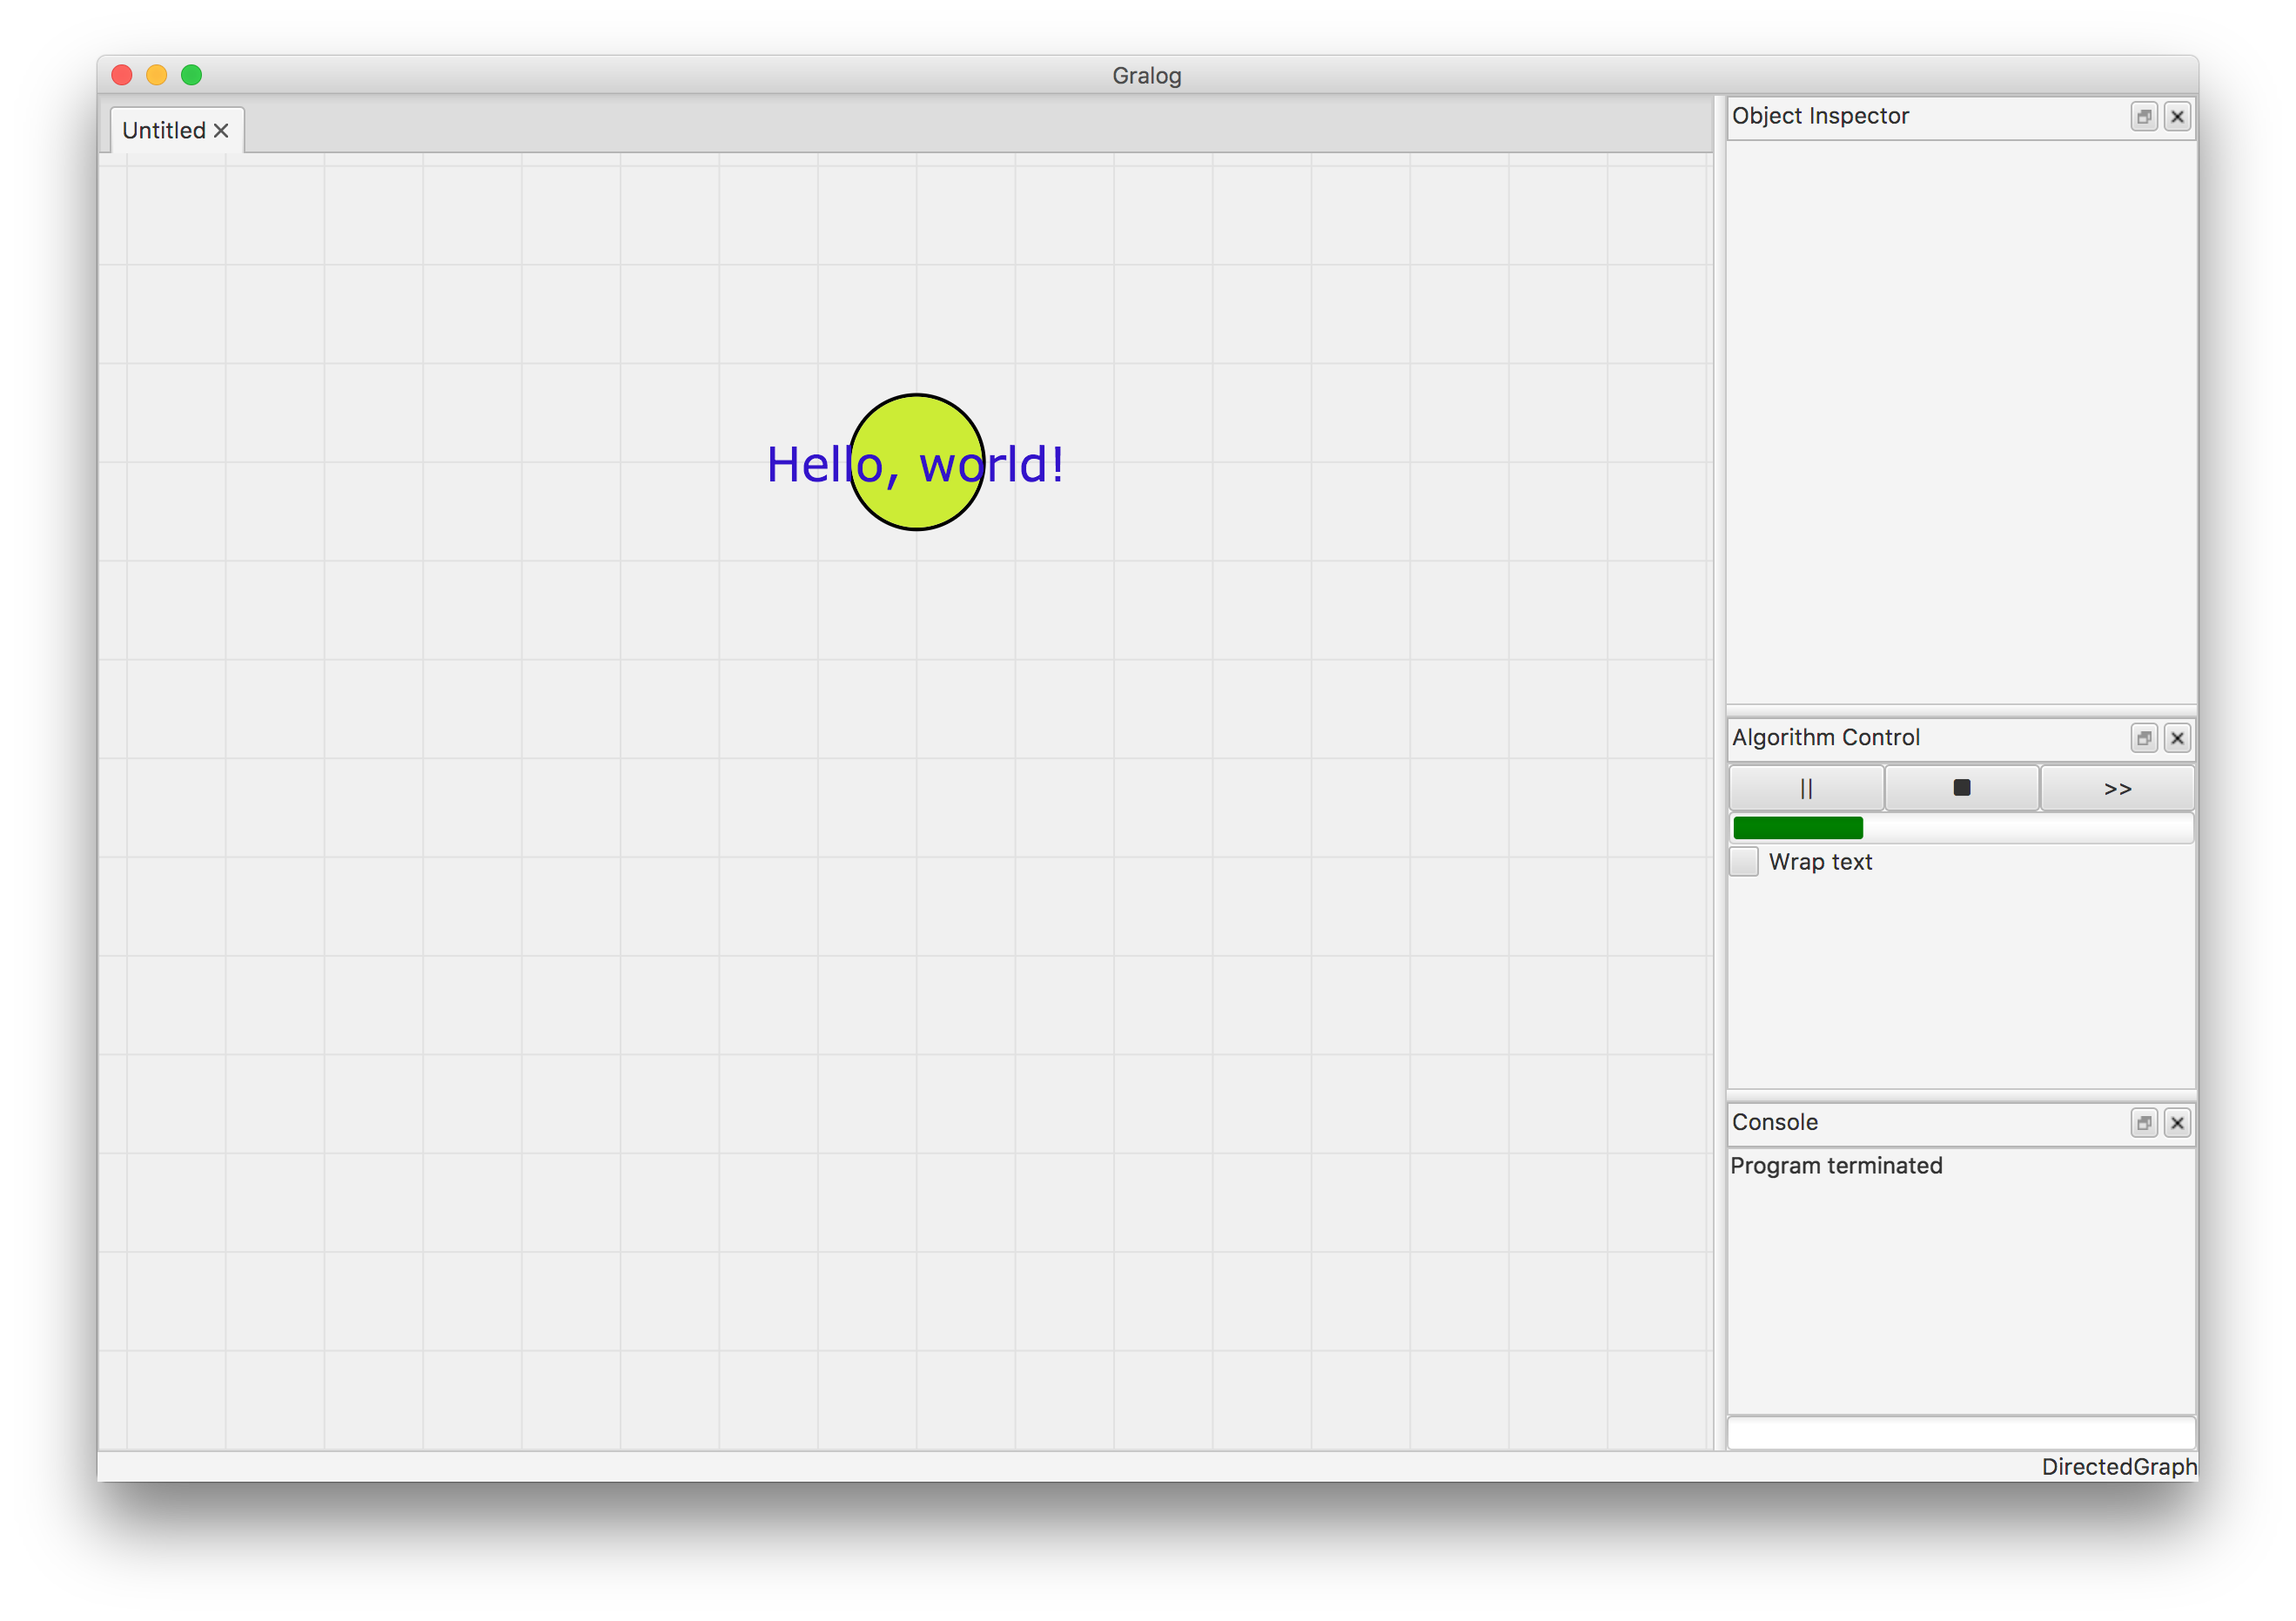
\includegraphics[width=\textwidth]{helloWorld.png}
\end{figure}

\subsection{Troubleshooting}
First obviously make sure you have python installed (version 2.7). Also make sure that Lib.py is in the directory as the file you wish to execute. Obviously you can mess around with the file structure to fit your needs but in this configuration they must be in the same directory. For other outstanding problems feel free to shoot an email at felix.herron@gmail.com 

\section{Introduction}
Now that you have the code running and set up, what will follow is a brief explanation of all of the functionality which we have built, structured in an intuitive manner.

\subsection{The Graph Class}
The first relevant class is Graph. In every program, you must choose a graph on which to execute your program. This is accomplished by instantiating the class Graph. 

\begin{lstlisting}
g = Graph();
\end{lstlisting}

In the constructor you specify which type of graph you would like. No argument means use the graph that is currently opened, whatever (type) it may be.

The Graph class can be seen as the moderator of the program. You will use it to do all of the surface-level, more general commands pertaining to the graph itself. The more intricate details will be done using the following two:

\subsection{The Vertex Class}
Each vertex is represented as an object of the class Vertex. It is distinguished by its unique ID. 

\begin{lstlisting}
v = g.createVertex();
\end{lstlisting}

All methods pertaining to the individual vertices, such as their color, neighbours, or label, are most easily manipulated using methods of this class. For example:

\begin{lstlisting}
v = g.createVertex(id=42);
v.setLabel("f00");
neighbours = v.getNeighbours();
myLabel = v.getLabel();
v.delete();
\end{lstlisting}

\subsection{The Edge Class}
Each edge is represented as an object of hte Edge class. It is distinguished by its unique ID; however, in graphs without multi-edges, it can also be distinguished by its source and target vertices.

\begin{lstlisting}
e = g.createEdge(v1,v2,directed=False);
\end{lstlisting}

All methods pertaining to the individual edges, such as their color, adjacent edges, or label, are most easily manipulated using methods of this class. For example:

\begin{lstlisting}
e = g.createEdge(v1,v2,directed=False,id=451);
e.setLabel("f00");
adjacentEdges = e.getAdjacentEdges();
target = e.getTarget();
e.delete();
\end{lstlisting}

The documentation will now simply elaborate on these concepts.

\section{Documentation}

\subsection{Class Graph}

\textbf{{\large Instance Variables}}

\begin{table}[h]
\begin{tabular}{p{\q}p{\q}}
Instance Variable & Meaning and Usage \\ \hline
\textbf{Dictionary} \textit{vertices} & A dictionary that holds all of the Vertex objects known to the graph. This should ideally not be changed by the programmer \\\hline
\textbf{Dictionary} \textit{edges} & A dictionary that holds all of the Edge objects known to the graph. This should ideally not be changed by the programmer \\\hline
\textbf{Integer} \textit{id} & The id of the graph that is used in communication with gralog. This should ideally not be changed by the programmer \\ \hline
\textbf{Dictionary} \textit{variablesToTrack} & Objects in format (name,value). These are displayed in the Algorithm Control Panel during pauses. These may be changed \\ \hline
\textbf{Dictionary} \textit{variablesToTrack} & Objects in format (name,value). These are displayed in the Algorithm Control Panel during pauses. These may be changed \\ \hline
\end{tabular}
\end{table}

\textbf{{\large Relevant Methods}}
\textit{Note: optional parameters are in parentheses}

\begin{table}[h]
\begin{tabular}{m{\smallCol}m{\argsLen}m{\smallCol}m{\q}}
Method & Arguments & Returns & Description \\ \hline
\textbf{Graph}& (str: format) & Graph Object & Returns a graph object. The parameter options are either nothing, ``directed'',``undirected'',``buechi'',``kripke'',``automaton'' \\\hline
\\\multicolumn{4}{c}{\textbf{Graph Manipulating Methods}}\\\\\hline
\textbf{addVertex}  & \makecell{(int: x)\\(int: y)\\(int: vertexId)} & \textbf{Vertex} object & creates a new Vertex object. If no coordinates passed, random coordinates are chosen. If no id is passed, a suitable id is chosen. If an id is passed that has already been assigned, a suitable new one is chosen\\\hline
\textbf{deleteVertex} & Vertex Object or id of vertex & void & Deletes the vertex or the vertex with the given id from the graph\\ \hline
\textbf{addEdge} & \makecell{Vertex: sourceVertex\\Vertex: targetVertex\\(Boolean: directed) \\ (int: edgeId)} & \textbf{Edge} object & creates a new Vertex object from the source vertex to the target vertex. If directed is not specifeed, un-directed is assumed. If un-directed, the order of target and source vertex is irrelevant. If no id is passed, a suitable id is chosen. If an id is passed that has already been assigned, a suitable new one is chosen \\ \hline
\textbf{addDirectedEdge} & \makecell{Vertex: sourceVertex\\Vertex: targetVertex \\ (int: edgeId)} & \textbf{Edge} object & calls addEdge with directed=True \\ \hline
\textbf{deleteEdge} & Edge object or id of edge & void &  Deletes the edge or the edge with the given id from the graph\\ \hline
\textbf{deleteAllEdges} & void & void & removes all edges from the graph \\ \hline
\\\multicolumn{4}{c}{\textbf{Setter Functions}}\\\\\hline
\textbf{setVertexFillColor} & \makecell{Vertex: vertex\\(str: colorHex)\\(int,int,int): colorRGB)} & void & sets the \textit{fill} color of the given vertex to the Hex code color specified or the RGB color specified. colorHex can also be a string of a common collor, such as "red" or "green."  \\ \hline
\textbf{setVertexStrokeColor} & \makecell{Vertex: vertex\\(str: colorHex)\\(int,int,int): colorRGB)} & void & sets the \textit{stroke} color of the given vertex to the Hex code color specified or the RGB color specified. colorHex can also be a string of a common collor, such as "red" or "green."  \\ \hline
\end{tabular}
\end{table}




\end{document}
